\documentclass[12pt,a4paper]{amsart}
\usepackage[utf8]{inputenc}
\usepackage{amsmath}
\usepackage{amsfonts}
\usepackage{amssymb}

\usepackage{hyperref}

\usepackage{float}
\usepackage{subfig}


%\usepackage[dvipdfmx]{graphicx}
\usepackage{graphicx}
\usepackage{caption}
%\usepackage[nobysame, alphabetic]{amsrefs}
%\usepackage{here}
%\usepackage{showkeys}
\newcommand{\modif}{$\clubsuit$}
\newtheorem{thm}{Theorem}[section]
\newtheorem{defn}[thm]{Definition}
\newtheorem{coro}[thm]{Corollary}
\newtheorem{prop}[thm]{Proposition}
\newtheorem{lem}[thm]{Lemma}
%\theoremstyle{definition}
\newtheorem{rmk}[thm]{Remark}
\newtheorem{cond}[thm]{Condition}

%CB defs
\def\HH{\mathbb{H}}
\def\dHH{\partial \mathbb{H}}
\def\HHn{\HH^n}
\def\hd{\hat{\delta}}
\def\ha{\hat{\alpha}}
\def\haa{\ha \cup \{\alpha^+,\alpha^-\}}

\def\im{\mathrm{Im}\,}



\def\gx{\Gamma(2)}
\def\xx{\HH/\Gamma(2)}
\def\gy{\Gamma_0(2)}
\def\xy{\HH/\Gamma_0(2)}


\def\ZZ{\mathbb{Z}}
\def\CC{\mathbb{C}}
\def\RR{\mathbb{R}}
\def\QQ{\mathbb{Q}}
\def\NN{\mathbb{N}}

\def\tt{\Sigma_{1,1}}

\def\fp{\mathbb{F}_p}
\def\aut{\text{Aut}(\F2)}
\def\gl2{\mathrm{GL}(2, \ZZ)}
\def\sl2{\mathrm{SL}(2, \ZZ)}
\def\sln{\mathrm{SL}(2, \ZZ/n\ZZ)}

\def\gg{\mathcal{G}_n}
\def\ggp{\mathcal{G}_p}

\def\isom{\mathrm{isom}(\HH)}

\def\isomH{\text{isom}^+(\HH)}
\def\tr{\text{tr\,}}


\def\GI{\mathbb{Z}[i]}
\def\hc{\CC \setminus \GI}



\title{Quadratic forms and  congruence subgroups}

 \author[McShane]{Greg McShane}
\address{Institut Fourier 100 rue des maths, BP 74, 38402 St Martin d'H\`eres cedex, France}
\email{mcshane at univ-grenoble-alpes.fr}


\begin{document}

\maketitle

\begin{abstract} 
	The  primes $p$  represented by a quadratic fors 
	$x^2 + y^2$, 
	$x^2 + 2y^2$, 
	$x^2 + 3y^2$, 
	is a subject that was first  studied by Fermat. 
	Heath-Brown and Zagier 
\end{abstract} 


\section{Introduction}

Consider the following pair of well known theorems from elementary number theory:



\begin{thm}[Fermat]\label{main}
Let $p$ be a prime then the equation
$$x^2 + y^2 = p $$
has a solution in integers  iff  $p =2$ or $p-1$ is a multiple of $4$.
\end{thm}

These results are intimately linked and often one deduces the second as a corollary of the first,
 for example, by using unique factorisation in the Gaussian integers.  
 We present a  geometric  approach to this results  using the theory of group actions and in particular an application of Burnsides's Lemma. 
 We also investigate this approach applied to the forms $x^2 + 2y^2$ and $x^2 + 3y^2$.
 
 
As in Zagier's remarkable proof \cite{zagier} both results follow from showing that a certain involution has a fixed point. 
Amusingly Burnsides's Lemma reduces this to showing that another involution has exactly two fixed points:
\begin{itemize}
\item  In the proof of Theorem \ref{triv} this is a consequence of the fact that a quadratic equation 
over a field has at most two solutions.
\item In the proof of Theorem \ref{main} this follows from some geometry and the fact that 
	any odd integer can be written as the difference of two squares.
 \end{itemize}


\subsection{Organisation, Remarks}

In Section 2 we recall the statement of Burnsides Lemma 
and apply it to a Klein four group generated by involutions of $\fp^*$
yielding a proof of Theorem \ref{triv}. 
In Section 3  we  introduce the  congruence subgroups and involutions involved.
In Section 4 we study how the involutions act on arcs and give explicit computations.  
Finally in Sections 5  and 6  we prove the main technical result and show how it is applied
to the quadratic forms $x^2 + y^2$, $x^2 + 2y^2$ and $x^2 + 3y^2$.


\subsubsection{References}
The reader should not need any other references to understand 
this paper if they are already familiar with  Burnsides Lemma.
For background the book by Cox \cite{cox} is highly recommended.

\subsubsection{Burnside and signatures}
 The astute reader will surely realise that Burnside is not essential to our argument
 and that one can achieve the same reduction by considering the signature
 of the permutations associated to the  involutions we consider. 
 In fact the first author set this as an  undergraduate exam question some years ago.
 
% \subsubsection{Lambda lengths}
%  The idea of associating a length to a geodesic joining cusps
%  (paragraph \ref{lengths}) appears in Penner's work on moduli \cite{bob}.
% He defined the $\lambda$-length of simple bicuspidal geodesic 
% on a punctured
% surface to be the length of the portion outside of some fixed
%  system of cusp regions.
 
 
 \subsubsection{Bezouts Theorem}
 In previous work \cite{vlad} we were implicitly using  Bezout's Theorem
 when we assert that
 \begin{itemize}
 \item $\sl2$ is transitive on $\QQ \cup \infty$ (which is equivalent to Bezout's Theorem.)
 \item $\Gamma(2) $ has exactly three orbits on $\QQ \cup \infty$.
 \end{itemize}
 We  will see in Section \ref{arcs and involutions} how to determine  the actions 
 of the various involutions explicit using Bezout's Theorem.
 
\subsection{Thanks}

The first author thanks Louis Funar and the second author for  many useful conversations over the years concerning this subject. He would also like to thank Xu Binbin for reading early drafts of the manuscript.


\section{Burnside Lemma}

Recall the following result from elementary number theory
\begin{thm}\label{triv}
Let $p$ be a prime then the equation
$$x^2 = -1$$
admits a solution in $\fp$ iff 
$p =2$ or $p-1$ is a multiple of $4$.
\end{thm}

We give a proof of this using the Burnside Lemma.


Recall that if $G$ is  a group acting on a finite set $X$ then the Burnside Lemma says
\begin{equation}\label{burnside}
|G| |X/G| = \sum_{g} |X^g| 
\end{equation}  
where, as usual, 
 $X^g$ denotes the set of fixed points of the element $g$ 
 and $X/G$  the orbit space.


Let $p\neq 2$,  $X = \fp^*$ and $G$ be the group generated by the two involutions
\begin{eqnarray*}
x & \mapsto -x \\
x & \mapsto 1/x.
\end{eqnarray*}
The group  $G$ has exactly four elements namely:
\begin{itemize}
\item the trivial element which has  $p-1$ fixed points
\item $x\mapsto -x$ which has no fixed points 
\item  $x\mapsto 1/x$ has exactly two fixed points namely $1$ and $-1$.
\item  $g:x \mapsto -1/x$ is the remaining element and the theorem is equivalent to the existence of a fixed point for it.
\end{itemize}
Note that since $\fp$ is a field 
$|X^g| = \sharp \{x^2 = -1, \, x\in \fp^* \}$
is either $0$ or $2$.
Now for our choice of $X$ and $G$ equation (\ref{burnside}) yields
\begin{equation}
4 |X/G|   = (p-1) + 2 + |X^g|.
\end{equation}  
The LHS is always divisible by $4$ so the  RHS is too and
it follows from this that
$$ |X^g|. = \left\{  \begin{array}{ll}
0 & (p-1) =  2 \mod 4 \\
2 & (p-1) =  0 \mod 4 \\
\end{array}
\right.
$$
This proves Theorem \ref{triv}.

\subsection*{Note}
As was noted in the introduction one can obtain the same conclusion 
by calculating the signature of $x\mapsto -1/x$ 
using the fact that it is  the composition of
$x \mapsto -x$ and $x \mapsto 1/x$.




% $$\begin{pmatrix}
% a & b \\
% c & d
% \end{pmatrix} \in \sl2,\, z\in \HH,\, 
% \begin{pmatrix}
% a & b \\
% c & d
% \end{pmatrix}. z = \frac{az + b}{cz + d}.
% $$

% The quotient $\xx$ is conformally equivalent to the Riemann  sphere minus three points
% which we will refer to as \textit{cusps}
% (see Figure \ref{3punctured}). 
% Following  convention we label these cusps $0,1,\infty$ respectively
% corresponding to the three $\gx$ orbits of $\QQ \cup \infty$. 
% Finally, the \textit{standard fundamental domain}  for $\gx$ 
% is the convex hull of the points $\infty, -1, 0 , 1$.
% This region can be decomposed into two ideal triangles 
% $\infty, -1, 0 $ and $ 0 , 1,\infty$ as in Figure \ref{fund}.
% The edges of the ideal triangles project to three disjoint simple geodesics on $\xx$
% and each edge has a \textit{midpoint} 
% which is a point of the $\sl2$ orbit of $i$ (see Figure \ref{3punctured}).

% \begin{figure}[hb]
% \begin{center}
% 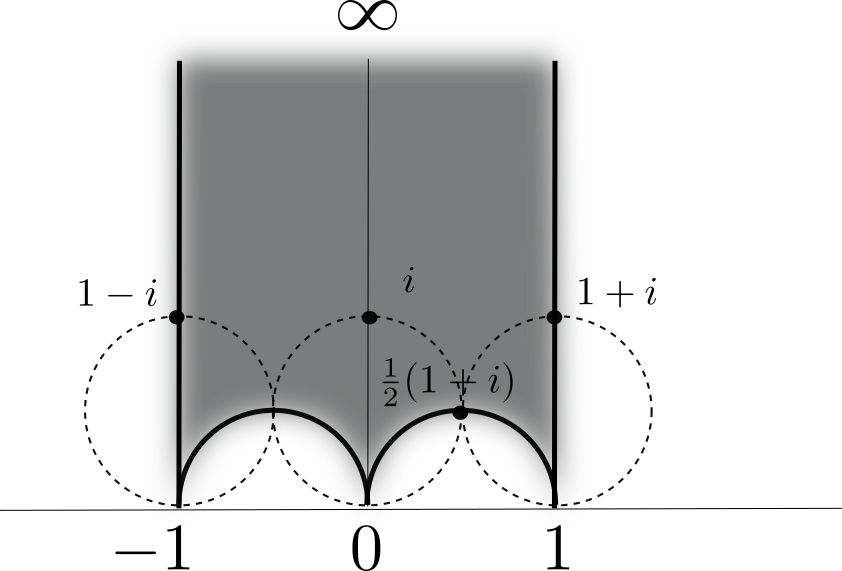
\includegraphics[scale=.5]{fund_dom.png} 
% \end{center}
% \caption{Standard fundamental domain for $\gx$ and its decomposition into ideal triangles.}
% \label{fund}
% \end{figure}


\section{Congruence subgroups}

We denote by  $\Gamma$ the  group of invertible matrices with integer coefficients  $\sl2$ 
and  define  $\Gamma(n)$ to be the 
kernel of the  homomorpisms $\sl2 \mapsto \sln$. 
The  latter group  is  a subgroup  of $\Gamma_0(n)$ 
$$ \left \{  \begin{pmatrix} a & b \\ c & d \end{pmatrix} \in \sln \, ,  c  =  0  \mod p \right \}. $$

\begin{figure}[hb]
\begin{center}
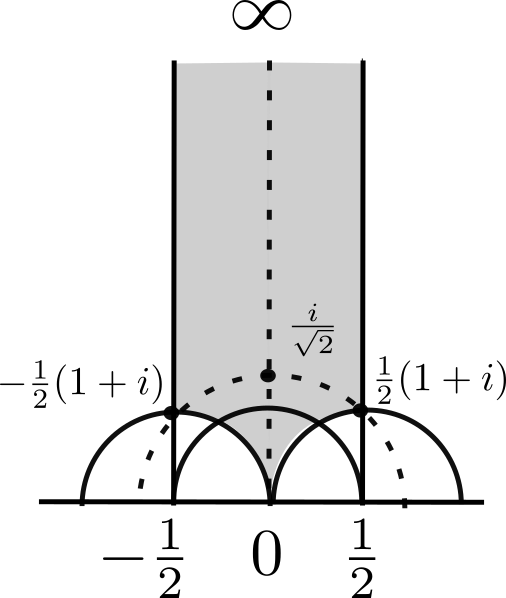
\includegraphics[scale=.5]{fund_dom2.png} 
\end{center}
\caption{Standard fundamental domain for $\Gamma_0(2)$}
\label{fund}
\end{figure}

It  is  well  known  that the involution 
$$  \tau_n  = \begin{pmatrix} 0 & -1/\sqrt{n} \\ \sqrt{n} &  0  \end{pmatrix} $$
normalises  $\Gamma_0(n)$.


For $n = 2,3$  or $4$ it is easy to find a fundamental domain for the  group
$\Gamma^*$ generated by $\tau_n$ and  $\Gamma_0(n)$. Let $U$ denote the strip
between the Poincare  geodesics (vertical lines) joining $\infty$ to $\pm
\frac12$ and $V_n$  the image of this strip under $\tau_n$ this is easy to
compute and it  is the region between the pair of Poincare  geodesics joining
$0$ to $\pm \frac{2}{n}$. 
The  region $U$ is the standard fundamental domain

The  intersection $U \cap V_n$ contains a fundamental
domain for $\Gamma^*$. 
For  $n = 2, 3, 4 $ this intersection is finite area and is a fundamental  domain for $\Gamma_0(n)$ with side pairings $P$ and $Q$.
The Poincare geodesic $\mu_n$ joining $-2/n$ to $2/n$ divides it into two regions each
of which is a fundamental domain for $\Gamma^*$.


From covering theory, an isometry  of $\HH$ 
induces an automorphism of  the  surface $\HH / G$ iff it normalises the covering group
i.e. $G$.
The fundamental domain for $\Gamma_0(n)$ is 
invariant under the  pair of orientation  reversing involutions 
$$ z \mapsto -\bar{z} ,\, z \mapsto \frac{1}{\bar{nz}} $$
and these maps preserve side pairings so normalise  $\Gamma_0(n)$.
One checks that their composition coincides with $\tau_n$.
Thus these three involutions together with the identity form a Klein four group 
that  normalises $\Gamma_0(n)$.

\begin{figure}[hb]
\begin{center}
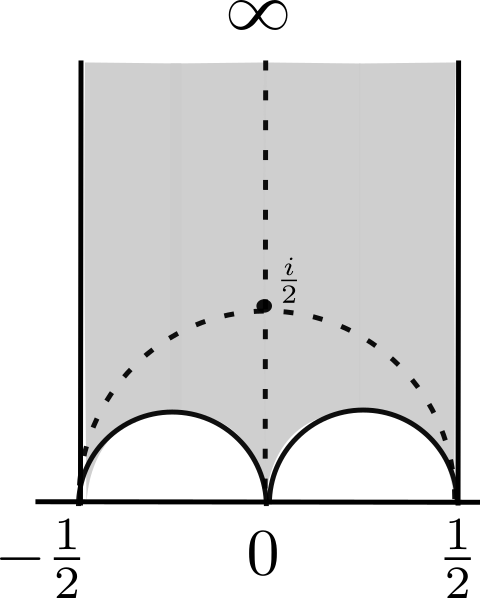
\includegraphics[scale=.5]{fund_dom4.png} 
\end{center}
\caption{Standard fundamental domain for $\Gamma_0(4)$}
\label{fund4}
\end{figure}


\section{Arcs and involutions}\label{arcs and involutions}

There is  a natural map from the set of coprime integers into the rationals
namely: $$(p,q) \mapsto \frac{p}{q}.$$ This map can be extended to be a
surjection onto the extended rationals $\QQ \cup \infty$ by $$(1,0) \mapsto
\infty.$$ 
The modular group $\Gamma$ acts transitively on $\QQ \cup \infty$ and
the stabiliser of $\infty$ is generated by the parabolic $z\mapsto z+1$.
Since  $\Gamma_0(n)$ is finite index in $\Gamma$ the extended
rationals is exactly the set of fixed points of the parabolic elements of
$\Gamma_0(n)$.

We define an \textit{arc} to be a Poincare  geodesic joining  distinct points of $p/q ,\,  p'/q' \in \QQ \cup \infty$.	
To each such arc we associate 
an 2x2 matrix  with integer coefficients:
$$\begin{pmatrix} p & p' \\ q  & q' \end{pmatrix}.$$

We will be concerned with the action of our Klein four group on the set 
set of geodesics joining $\infty$ to a point $k/q$  where  $q$ is some prime.
The corresponding matrices have the form
$$\begin{pmatrix} 1 & k  \\ 0  & q \end{pmatrix}.$$
We can compute the action of $\tau_n$ on `the  endpoints of an  arc:
\begin{eqnarray*}
\infty  \mapsto 0, \, k/q \mapsto -q/nk
\end{eqnarray*}
so the correspondng arc has matrix
$$\begin{pmatrix} 0 & -q  \\ 1  & nk \end{pmatrix}.$$

Since $q$ and $nk$  are coprime there exist integers $a$ and $b$ such that
$bnk + aq = 1$.
And so the matrix
$$\begin{pmatrix} a & -b  \\ nk  & q \end{pmatrix}$$
is in $\Gamma_0(n)$.

Now we have:
$$\begin{pmatrix} a & -b  \\ nk  & q \end{pmatrix}
\begin{pmatrix} 0 & -q  \\ -1  & nk \end{pmatrix}
= \begin{pmatrix} -b & -aq -bnk  \\ q   & 0 \end{pmatrix}
= \begin{pmatrix} -b & -1 \\ q   & 0 \end{pmatrix}
.$$

So the action of $\tau_n$ on the set of arcs can be computed using the euclidean algorithm to find $b$.


\subsection{Explicit computations for $n=2$ and  $p = 7,11$}

We will compute the action of $\tau_2$ on the set of arcs joining $\infty$ to a point $k/7$ or $k/11$.
For $k = 1,2,3 \ldots p-1$ we denote $k'/p$   the image  of $k/p$ under $\tau_2$

So for $p=7$  we have:
\begin{center}
\begin{tabular}{|c|c|c|c|c|c|c|}
	\hline
	k& 1 & 2 & 3 & 4 & 5 & 6 \\ 
\hline
	k'&-4 & -2 & 1 & -1 & 2 & -3
\\  \hline
\end{tabular}

\end{center}


So for $p=11$  we have:
\begin{center}
\begin{tabular}{|c|c|c|c|c|c|c|c|c|c|c|}
\hline
k& 1 & 2 & 3 & 4 & 5 & 6 & 7 & 8 & 9 & 10 \\ 
\hline
k'& -6 & -3 & -2 & 4 & 1 & -1 & -4 & 2 & 3 & -5
\\  \hline
\end{tabular}
\end{center}


\section{Invariant arcs and solutions to $x^2  \pm n y^2 = p$}\label{fixed points}

\begin{thm}\label{fixed points theorem}
Let $n$ be a positive integer and $p$ a prime:
\begin{enumerate}
	\item 
$$ x^2 + n y^2 =p $$
has a solution iff $\tau_q$ 
leaves one of the arcs joining $\infty$ to $k/p$ invariant;

	\item $$ x^2 - n y^2 =p $$
has a solution iff the involution $z \mapsto 1/(n \bar{z})$ 
leaves one of the arcs $\infty$ to $k/p$ invariant;
\end{enumerate}


\end{thm}

\begin{proof}
Suppose there is an arc joining $a/b$ to $a'/b'$ that is invariant under $\tau_n$.
Then $a' = -b$ and $b' = n a$ since 
$$\tau_n(a/b) = \frac{-1}{n(a/b)} = \frac {-b}{na}.$$
So the matrix corresponding to the arc is (up to permuting the columns)
$$\begin{pmatrix} a & -b  \\ b  & n a \end{pmatrix}.$$
If this arc is equivalent  by an element of $\Gamma_0(n)$ to an arc of the form
$\infty \to k/p$ ie  whose matrix is 
$$\begin{pmatrix} 1 & k  \\ 0  & p  \end{pmatrix}.$$
for some $k$ then the determinant of the associated matrix,
that is $b^2 +n a^2$, is $ p$.

The enuation  $x^2 + n y^2 =p$ is proven in a similar way.
\end{proof}


\section{Existence of solutions to $x^2 \pm n y^2 = p$}\label{existence}	

Let $p$ be an odd prime.

\subsection{The case $x^2 + 4 y^2 = p$}\label{case 1}

This is Fermat's result from the introduction.	
We will prove that the equation has a solution iff $p \equiv 1 \pmod{4}$.

If $p = 4k+1$ then there is an (essentially unique) solution to $x^2 + 4 y^2 = p$.
The involution $z \mapsto 1/4 \bar{z}$ actually leaves a pair of arcs invariant 
One can  see this  from the theorem
and the fact that
$$x^2 - 4 y^2  = (x -2y)(x+2y).$$
Since $p$  if $p = x^2 - 4y^2$ then
$x-2y = 1$ and $x+2y = p$ so $x = (p+1)/2$ and $y = (p-1)/4$.

Now applying our argument with the Burnside Lemma we see that $\tau_4$ leaves a pair of arcs invariant so there are  solutions to $x^2 + 4 y^2 = p$.



\subsection{The case $x^2 + 2 y^2 = p$}\label{case 1}

If $p$ can be written as $8k+1$ or $8k+3$ then there is a solutions to $x^2 + 2 y^2 = p$.

The case $8k+3$ follows from the argument with Burnside again. The involution $z \mapsto 1/2 \bar{z}$ leaves no arc invariant.
By the theorem this is equivalent to saying that there is $p$ cannot be written as $x^2 - 2 y^2$ and this is easy to prove using congruences mod $8$.	

Reciprocally $p= 8k+7$ can be written as $x^2 - 2 y^2$  as it cannot be written as $x^2 + 2 y^2$.

Unfortunately the case $p = 8k+1$ is not so easy. There seems to be no way to deduce this by using a parity argument
although Generalov  \cite{Generalov}  does claim to have a  proof using involutions.

\thebibliography{99}
\bibitem{cox}
David A. Cox
Primes of the Form $x^2 + ny^2$: Fermat, Class Field Theory, and Complex Multiplication, Second Edition
2013 John Wiley & Sons

% \bibitem{ford}
% Lester R Ford,
% \textit{Automorphic Functions}

\bibitem{Generalov}
Generalov, A.I. 
A combinatorial proof of Euler-Fermat’s theorem on the representation of the primes $ p=8k+3$ by the quadratic form $x^2+2y^2$ . J Math Sci 140, 690–691 (2007).

\bibitem{thesis}
G. McShane,
\textit{Simple geodesics and a series constant over Teichmuller space}
Invent. Math. (1998)

% \bibitem{mong}
% M.L. Lang, S.P Tan,
% \textit{A simple proof of the Markoff conjecture for prime powers}
% Geometriae Dedicata volume 129, pages15–22 (2007)

\bibitem{bob}
R. C. Penner, 
\textit{The decorated Teichmueller space of punctured surfaces}, 
Communications in Mathematical Physics 113 (1987), 299–339.


% \bibitem{serre}
% J-P. Serre,
% \textit{A Course in Arithmetic},
% Graduate Texts in Mathematics,
% Springer-Verlag New York
% 1973

% \bibitem{saw}
% Scott Wolpert,
% \textit{On the Kahler form of the moduli space of once-punctured tori}, 
% Comment. Math. Helv. 58(1983)246-256

\bibitem{zagier}
D. Zagier,
 \textit{A one-sentence proof that every prime p = 1 (mod 4) is a sum of two squares}, 
 American Mathematical Monthly, 97 (2): 144
 
 % \bibitem{zhang}
 % Y. Zhang,
 % \textit{ An elementary proof of uniqueness of Markoff numbers}
 % preprint, arXiv:math.NT/0606283
 
  % \bibitem{zhangx}
  %  Y. Zhang,
 % \textit{Congruence and uniqueness of certain Markoff numbers}
 % Acta Arithmetica, Volume: 128, Issue: 3, page 295-301







 



\end{document}


